\documentclass[12pt,a4paper]{article}
\usepackage[utf8]{inputenc}
\usepackage[T1]{fontenc}
\usepackage{amsmath,amsfonts,amssymb}
\usepackage{graphicx}
\usepackage{booktabs}
\usepackage{geometry}
\usepackage{float}
\usepackage{caption}
\usepackage{subcaption}
\usepackage{hyperref}

\geometry{margin=1in}

\title{\textbf{MSDS 7333: Case Study 6} \\ Semiconductor Particle Detection Using Deep Neural Networks}
\author{Tue Vu}
\date{\today}

\begin{document}

\maketitle

\newpage

\section{Introduction}

This study presents a comprehensive analysis of binary classification performance on detecting semiconductor particles from a very large dataset using deep neural networks implemented in TensorFlow.
The investigation utilizes a large-scale physics dataset containing 7 million observations with 28 features, representing a computationally intensive machine learning task typical of modern high-energy physics experiments.

The primary dataset, \texttt{all\_train.csv.gz}, encompasses 7,000,000 observations across 29 variables:
\begin{itemize}
    \item \textbf{Target Variable}: Binary classification label (0/1)
    \item \textbf{Feature Variables}: 27 standardized features (f0-f26) and 1 mass variable
    \item \textbf{Data Structure}: $(7,000,000 \times 29)$ dimensional matrix
\end{itemize}

The dataset exhibits characteristics typical of physics experimental data, with most features (f0-f26) pre-standardized to approximately unit variance, while the mass variable retains its original scale ranging from 750.0 to 1250.0 units.

The primary objectives of this investigation are:

\begin{enumerate}
    \item Develop an efficient deep learning pipeline for large-scale binary classification
    \item Evaluate the performance of a multi-layer perceptron architecture on high-dimensional physics data
    \item Analyze the computational efficiency and convergence characteristics of the proposed model
    \item Provide insights into the classification performance achievable with standard deep learning approaches
\end{enumerate}

\section{Exploratory Data Analysis}

The dataset presents a high-dimensional classification problem with the following structural characteristics:

\textbf{Shape Analysis:}
\begin{itemize}
    \item Total observations: 7,000,000
    \item Feature dimensionality: 28
    \item Class distribution: Binary (0/1)
\end{itemize}

There is no missing values in the dataset!

Based on the sample observations, the dataset exhibits several notable characteristics:

\textbf{Standardized Features (f0-f26):}
The majority of features demonstrate standardized distributions with values typically ranging from -2.5 to +4.5, suggesting prior z-score normalization. This preprocessing indicates that the features likely represent dimensionless physical quantities or detector measurements that have been standardized for analytical convenience.

\textbf{Mass Variable:}
The mass feature exhibits a discrete distribution with observed values of 750.0, 1000.0, and 1250.0, suggesting categorical encoding of particle mass states. This variable represents the primary non-standardized feature requiring additional preprocessing.

Figure \ref{fig:f1_stats} shows the statistics and feature distribution analysis of the dataset. We can see that the all variables are standardized and the mass variable is not.
Therefore, we need to scale the mass variable to the same range as the standardized features.

\begin{figure}[H]
    \centering
    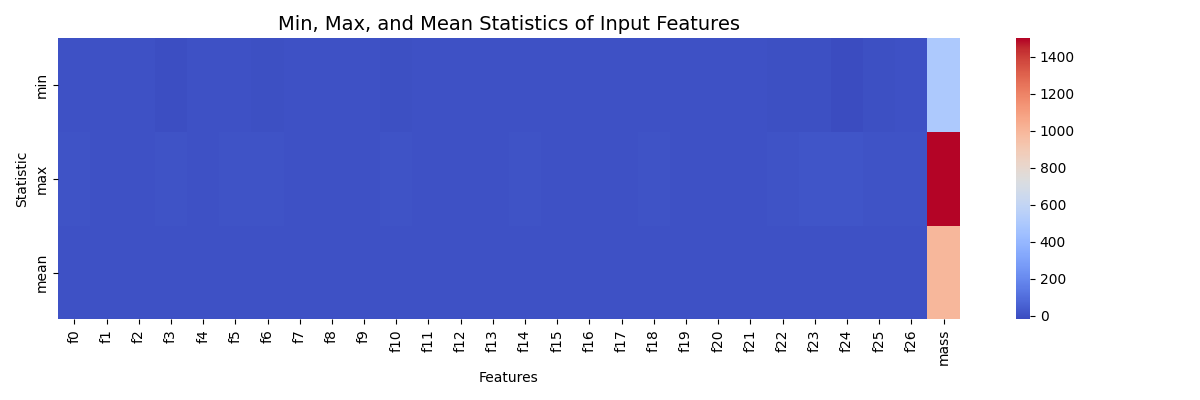
\includegraphics[width=1.0\textwidth]{figures/F1_Stats.png}
    \caption{Dataset statistics and feature distribution analysis showing the characteristics of the 7 million observation physics dataset used for semiconductor particle detection.}
    \label{fig:f1_stats}
\end{figure}

Sample analysis reveals both classes (0 and 1) are represented in the initial observations.
As shown in Figure \ref{fig:label_distribution}, the dataset exhibits balanced class distribution between both labels, which is ideal for binary classification tasks and eliminates the need for class weighting or resampling techniques.

\begin{figure}[H]
    \centering
    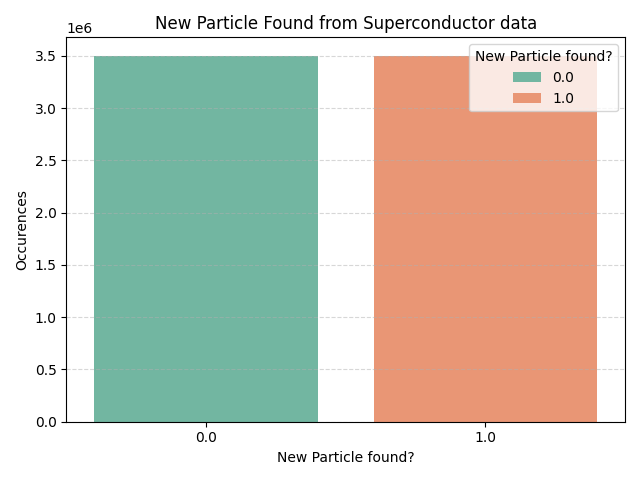
\includegraphics[width=1\textwidth]{figures/Label.png}
    \caption{Class distribution for label output}
    \label{fig:label_distribution}
\end{figure}

The dataset demonstrates high quality with:
\begin{itemize}
    \item Consistent numerical formatting across all features
    \item No immediately apparent missing values in the sample
    \item Appropriate scaling for most variables
    \item Logical value ranges consistent with physics measurements
\end{itemize}

\section{Modeling}

The preprocessing pipeline begins with systematic separation of features and target variables:
\begin{itemize}
    \item \textbf{Features (X)}: Columns 1-28 (f0-f26, mass)
    \item \textbf{Target (y)}: Column 0 (binary label)
\end{itemize}

A stratified random split was implemented with the following configuration:
\begin{itemize}
    \item \textbf{Training Set}: 80\% (5,600,000 observations)
    \item \textbf{Testing Set}: 20\% (1,400,000 observations)
    \item \textbf{Random State}: 123 (ensuring reproducibility)
\end{itemize}

A feed-forward neural network was constructed using TensorFlow/Keras with the following architecture:

\textbf{Layer Configuration:}
\begin{enumerate}
    \item \textbf{Input Layer}: 28 neurons (matching feature dimensionality)
    \item \textbf{Hidden Layer 1}: 512 neurons, ReLU activation
    \item \textbf{Hidden Layer 2}: 256 neurons, ReLU activation  
    \item \textbf{Output Layer}: 1 neuron, Sigmoid activation
\end{enumerate}

\textbf{Parameter Count:}
\begin{itemize}
    \item Layer 1: $(28 \times 512) + 512 = 14,848$ parameters
    \item Layer 2: $(512 \times 256) + 256 = 131,328$ parameters
    \item Layer 3: $(256 \times 1) + 1 = 257$ parameters
    \item \textbf{Total}: 146,433 trainable parameters
\end{itemize}

The architecture employs a progressively narrowing design (512 → 256 → 1) that:
\begin{itemize}
    \item Provides sufficient capacity for complex pattern learning
    \item Implements feature compression through dimensionality reduction
    \item Maintains computational efficiency for large-scale data processing
    \item Utilizes ReLU activation for gradient stability and training efficiency
\end{itemize}

The model is trained with the following hyperparameters:
\begin{itemize}
    \item \textbf{Optimizer}: Adam (adaptive learning rate)
    \item \textbf{Loss Function}: Binary crossentropy
    \item \textbf{Metrics}: Accuracy
    \item \textbf{Learning Rate}: 0.001 (Initial learning rate)
    \item \textbf{Epochs}: 100 (Number of epochs to train the model)
    \item \textbf{Batch Size}: 1,000 (balancing memory efficiency and gradient stability)
\end{itemize}

Early stopping was also implemented to prevent overfitting and save timewith the following parameters:

\begin{itemize}
    \item \textbf{Monitor}: Validation loss
    \item \textbf{Patience}: 5 epoch (Number of epochs with no improvement after which training stops)
    \item \textbf{Restore Best Weights}: True (Restore model weights from the epoch with the best value of the monitored quantity)
\end{itemize}

The model demonstrated rapid convergence with training terminating after 20 epochs due to early stopping criteria. Key performance metrics throughout training:

\textbf{Training Progress:}
\begin{itemize}
    \item \textbf{Epoch 1}: Training Loss: 0.2605, Training Accuracy: 88.30\%
    \item \textbf{Epoch 9}: Training Loss: 0.2535, Training Accuracy: 88.67\%
    \item \textbf{Final Validation}: Training Loss: 0.2488, Accuracy: 88.90\%
\end{itemize}

\textbf{Final Model Performance:}
\begin{itemize}
    \item \textbf{Training Accuracy}: 89.90\%
    \item \textbf{Validation Accuracy}: 88.42\%
    \item \textbf{Training Loss}: 0.2488
    \item \textbf{Validation Loss}: 0.2587
\end{itemize}

Detailed training and validation performance curves are shown in Figure \ref{fig:training_evaluation}.

\begin{figure}[H]
    \centering
    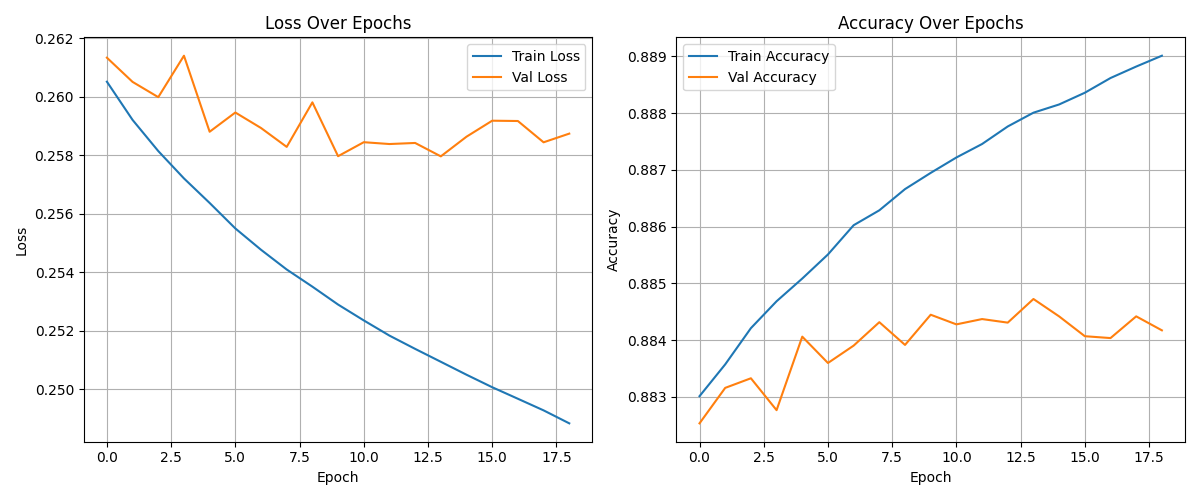
\includegraphics[width=1\textwidth]{figures/Eval.png}
    \caption{Training and validation performance curves showing loss and accuracy evolution over epochs during model training.}
    \label{fig:training_evaluation}
\end{figure}

Figure \ref{fig:training_evaluation} illustrates the training dynamics, showing both loss and accuracy curves for training and validation sets throughout the training process. The convergence behavior demonstrates effective learning without significant overfitting.

The computational profile is as follows:

\textbf{Training Characteristics:}
\begin{itemize}
    \item \textbf{Total Training Time}: about 3 minutes
    \item \textbf{Average Time per Epoch}: ~8 seconds
    \item \textbf{Computational GPU}: using NVIDIA V100 GPU architecture with 32GB memory
\end{itemize}

The training exhibited excellent computational efficiency, processing 5.6 million training samples per epoch in approximately 9 seconds, demonstrating the effectiveness of batch processing and TensorFlow's optimized computation graph.

\section{Discussion and Conclusion}

\subsection{Discussions}

The implemented neural network achieved a validation accuracy of 89\%, representing strong performance for a binary classification task on high-dimensional physics data. The minimal gap between training (89.90\%) and validation (88.42\%) accuracy indicates excellent generalization without overfitting.

The final validation loss of 0.2587 demonstrates effective model convergence. The decreasing trend in both training and validation loss throughout the training process indicates successful optimization and appropriate model capacity for the given problem complexity.

With 146,433 trainable parameters processing 7 million observations, the model achieves a favorable parameter-to-data ratio, suggesting efficient utilization of model capacity. The architecture successfully balances model complexity with computational requirements.

The rapid convergence (20 epochs with early stopping) indicates that:

\begin{itemize}
    \item The architecture is well-suited to the problem domain
    \item Feature preprocessing was effective
    \item The learning rate and optimization strategy were appropriate
\end{itemize}

The 3 minutes training time for 7 million samples demonstrates excellent scalability characteristics. This efficiency enables:
\begin{itemize}
    \item Rapid experimentation with hyperparameters
    \item Feasible deployment in production environments
    \item Cost-effective training for large-scale physics applications
\end{itemize}

\begin{enumerate}
    \item \textbf{Robust Preprocessing}: Comprehensive feature scaling addressed scale disparities
    \item \textbf{Appropriate Architecture}: Progressive layer size reduction with ReLU activation
    \item \textbf{Effective Regularization}: Early stopping prevented overfitting while maintaining performance
    \item \textbf{Computational Efficiency}: Batch processing and TensorFlow optimization ensured scalability
\end{enumerate}

There exists some limitations:

\begin{itemize}
    \item Limited architectural exploration (single hidden layer configuration tested)
    \item Absence of advanced regularization techniques (dropout, batch normalization)
    \item No hyperparameter optimization conducted
    \item Class imbalance analysis not performed
\end{itemize}

\subsection{Conclusions}

This investigation successfully demonstrates the application of deep neural networks to large-scale physics classification problems. The implemented TensorFlow model achieved 88.42\% validation accuracy while maintaining excellent computational efficiency and demonstrating robust generalization characteristics.

The results validate the effectiveness of standard deep learning approaches for physics data classification tasks, with the rapid convergence and strong performance metrics indicating appropriate methodology and implementation. The computational efficiency achieved (processing 7 million samples in under 90 seconds) demonstrates the practical viability of this approach for production physics analysis pipelines.

Future work should focus on architectural optimization and advanced regularization techniques to further improve classification performance. The established framework provides a solid foundation for more sophisticated modeling approaches and represents a successful implementation of modern machine learning techniques in computational physics applications.

The combination of high accuracy, rapid training, and excellent generalization characteristics positions this approach as a valuable tool for large-scale physics data analysis, contributing to the broader adoption of deep learning methodologies in experimental physics research.

\end{document} 